
%\documentclass[11pts,a4paper,amsmath,amssymb,floatfix]{article}%{report}%{book}
\documentclass[12pts,a4paper,amsmath,amssymb,floatfix]{article}%{report}%{book}
\usepackage{graphicx,wrapfig,pdfpages}% Include figure files
%\usepackage{dcolumn,enumerate}% Align table columns on decimal point
\usepackage{enumerate,enumitem}% Align table columns on decimal point
\usepackage{bm,dpfloat}% bold math
\usepackage[pdftex,bookmarks,colorlinks=true,urlcolor=rltblue,citecolor=blue]{hyperref}
\usepackage{amsfonts,amsmath,amssymb,stmaryrd,indentfirst}
\usepackage{times,psfrag}
\usepackage{natbib}
\usepackage{color}
\usepackage{units}
\usepackage{rotating}
\usepackage{multirow}


\usepackage{pifont}
\usepackage{subfigure}
\usepackage{subeqnarray}
\usepackage{ifthen}

\usepackage{supertabular}
\usepackage{moreverb}
\usepackage{listings}
\usepackage{palatino}
%\usepackage{doi}
\usepackage{longtable}
\usepackage{float}
\usepackage{perpage}
\MakeSorted{figure}
%\usepackage{pdflscape}


%\usepackage{booktabs}
%\newcommand{\ra}[1]{\renewcommand{\arraystretch}{#1}}


\definecolor{rltblue}{rgb}{0,0,0.75}


%\usepackage{natbib}
\usepackage{fancyhdr} %%%%
\pagestyle{fancy}%%%%
% with this we ensure that the chapter and section
% headings are in lowercase
%%%%\renewcommand{\chaptermark}[1]{\markboth{#1}{}}
\renewcommand{\sectionmark}[1]{\markright{\thesection\ #1}}
\fancyhf{} %delete the current section for header and footer
\fancyhead[LE,RO]{\bfseries\thepage}
\fancyhead[LO]{\bfseries\rightmark}
\fancyhead[RE]{\bfseries\leftmark}
\renewcommand{\headrulewidth}{0.5pt}
% make space for the rule
\fancypagestyle{plain}{%
\fancyhead{} %get rid of the headers on plain pages
\renewcommand{\headrulewidth}{0pt} % and the line
}

\def\newblock{\hskip .11em plus .33em minus .07em}
\usepackage{color}

%\usepackage{makeidx}
%\makeindex

\setlength\textwidth      {16.cm}
\setlength\textheight     {22.6cm}
\setlength\oddsidemargin  {-0.3cm}
\setlength\evensidemargin {0.3cm}

\setlength\headheight{14.49998pt} 
\setlength\topmargin{0.0cm}
\setlength\headsep{1.cm}
\setlength\footskip{1.cm}
\setlength\parskip{0pt}
\setlength\parindent{0pt}


%%%
%%% Headers and Footers
\lhead[] {\text{\small{EX3030/EM40JK}}} 
\rhead[] {{\text{\small{Tutorial: Transient HT and Heat Exchangers}}}}
%\chead[] {\text{\small{Session 2012/13}}} 
\lfoot[]{Dr Jeff Gomes}
%\cfoot[\thepage]{\thepage}
\rfoot[\text{\small{\thepage}}]{\thepage}
\renewcommand{\headrulewidth}{0.8pt}


%%%
%%% space between lines
%%%
\renewcommand{\baselinestretch}{1.5}

\newenvironment{VarDescription}[1]%
  {\begin{list}{}{\renewcommand{\makelabel}[1]{\textbf{##1:}\hfil}%
    \settowidth{\labelwidth}{\textbf{#1:}}%
    \setlength{\leftmargin}{\labelwidth}\addtolength{\leftmargin}{\labelsep}}}%
  {\end{list}}

%%%%%%%%%%%%%%%%%%%%%%%%%%%%%%%%%%%%%%%%%%%
%%%%%%                              %%%%%%%
%%%%%%      NOTATION SECTION        %%%%%%%
%%%%%%                              %%%%%%%
%%%%%%%%%%%%%%%%%%%%%%%%%%%%%%%%%%%%%%%%%%%

% Text abbreviations.
\newcommand{\ie}{{\em{i.e., }}}
\newcommand{\eg}{{\em{e.g., }}}
\newcommand{\cf}{{\em{cf., }}}
\newcommand{\wrt}{with respect to}
\newcommand{\lhs}{left hand side}
\newcommand{\rhs}{right hand side}
% Commands definining mathematical notation.

% This is for quantities which are physically vectors.
\renewcommand{\vec}[1]{{\mbox{\boldmath$#1$}}}
% Physical rank 2 tensors
\newcommand{\tensor}[1]{\overline{\overline{#1}}}
% This is for vectors formed of the value of a quantity at each node.
\newcommand{\dvec}[1]{\underline{#1}}
% This is for matrices in the discrete system.
\newcommand{\mat}[1]{\mathrm{#1}}


\DeclareMathOperator{\sgn}{sgn}
\newtheorem{thm}{Theorem}[section]
\newtheorem{lemma}[thm]{Lemma}

%\newcommand\qed{\hfill\mbox{$\Box$}}
\newcommand{\re}{{\mathrm{I}\hspace{-0.2em}\mathrm{R}}}
\newcommand{\inner}[2]{\langle#1,#2\rangle}
\renewcommand\leq{\leqslant}
\renewcommand\geq{\geqslant}
\renewcommand\le{\leqslant}
\renewcommand\ge{\geqslant}
\renewcommand\epsilon{\varepsilon}
\newcommand\eps{\varepsilon}
\renewcommand\phi{\varphi}
\newcommand{\bmF}{\vec{F}}
\newcommand{\bmphi}{\vec{\phi}}
\newcommand{\bmn}{\vec{n}}
\newcommand{\bmns}{{\textrm{\scriptsize{\boldmath $n$}}}}
\newcommand{\bmi}{\vec{i}}
\newcommand{\bmj}{\vec{j}}
\newcommand{\bmk}{\vec{k}}
\newcommand{\bmx}{\vec{x}}
\newcommand{\bmu}{\vec{u}}
\newcommand{\bmv}{\vec{v}}
\newcommand{\bmr}{\vec{r}}
\newcommand{\bma}{\vec{a}}
\newcommand{\bmg}{\vec{g}}
\newcommand{\bmU}{\vec{U}}
\newcommand{\bmI}{\vec{I}}
\newcommand{\bmq}{\vec{q}}
\newcommand{\bmT}{\vec{T}}
\newcommand{\bmM}{\vec{M}}
\newcommand{\bmtau}{\vec{\tau}}
\newcommand{\bmOmega}{\vec{\Omega}}
\newcommand{\pp}{\partial}
\newcommand{\kaptens}{\tensor{\kappa}}
\newcommand{\tautens}{\tensor{\tau}}
\newcommand{\sigtens}{\tensor{\sigma}}
\newcommand{\etens}{\tensor{\dot\epsilon}}
\newcommand{\ktens}{\tensor{k}}
\newcommand{\half}{{\textstyle \frac{1}{2}}}
\newcommand{\tote}{E}
\newcommand{\inte}{e}
\newcommand{\strt}{\dot\epsilon}
\newcommand{\modu}{|\bmu|}
% Derivatives
\renewcommand{\d}{\mathrm{d}}
\newcommand{\D}{\mathrm{D}}
\newcommand{\ddx}[2][x]{\frac{\d#2}{\d#1}}
\newcommand{\ddxx}[2][x]{\frac{\d^2#2}{\d#1^2}}
\newcommand{\ddt}[2][t]{\frac{\d#2}{\d#1}}
\newcommand{\ddtt}[2][t]{\frac{\d^2#2}{\d#1^2}}
\newcommand{\ppx}[2][x]{\frac{\partial#2}{\partial#1}}
\newcommand{\ppxx}[2][x]{\frac{\partial^2#2}{\partial#1^2}}
\newcommand{\ppt}[2][t]{\frac{\partial#2}{\partial#1}}
\newcommand{\pptt}[2][t]{\frac{\partial^2#2}{\partial#1^2}}
\newcommand{\DDx}[2][x]{\frac{\D#2}{\D#1}}
\newcommand{\DDxx}[2][x]{\frac{\D^2#2}{\D#1^2}}
\newcommand{\DDt}[2][t]{\frac{\D#2}{\D#1}}
\newcommand{\DDtt}[2][t]{\frac{\D^2#2}{\D#1^2}}
% Norms
\newcommand{\Ltwo}{\ensuremath{L_2} }
% Basis functions
\newcommand{\Qone}{\ensuremath{Q_1} }
\newcommand{\Qtwo}{\ensuremath{Q_2} }
\newcommand{\Qthree}{\ensuremath{Q_3} }
\newcommand{\QN}{\ensuremath{Q_N} }
\newcommand{\Pzero}{\ensuremath{P_0} }
\newcommand{\Pone}{\ensuremath{P_1} }
\newcommand{\Ptwo}{\ensuremath{P_2} }
\newcommand{\Pthree}{\ensuremath{P_3} }
\newcommand{\PN}{\ensuremath{P_N} }
\newcommand{\Poo}{\ensuremath{P_1P_1} }
\newcommand{\PoDGPt}{\ensuremath{P_{-1}P_2} }

\newcommand{\metric}{\tensor{M}}
\newcommand{\configureflag}[1]{\texttt{#1}}

% Units
\newcommand{\m}[1][]{\unit[#1]{m}}
\newcommand{\km}[1][]{\unit[#1]{km}}
\newcommand{\s}[1][]{\unit[#1]{s}}
\newcommand{\invs}[1][]{\unit[#1]{s}\ensuremath{^{-1}}}
\newcommand{\ms}[1][]{\unit[#1]{m\ensuremath{\,}s\ensuremath{^{-1}}}}
\newcommand{\mss}[1][]{\unit[#1]{m\ensuremath{\,}s\ensuremath{^{-2}}}}
\newcommand{\K}[1][]{\unit[#1]{K}}
\newcommand{\PSU}[1][]{\unit[#1]{PSU}}
\newcommand{\Pa}[1][]{\unit[#1]{Pa}}
\newcommand{\kg}[1][]{\unit[#1]{kg}}
\newcommand{\rads}[1][]{\unit[#1]{rad\ensuremath{\,}s\ensuremath{^{-1}}}}
\newcommand{\kgmm}[1][]{\unit[#1]{kg\ensuremath{\,}m\ensuremath{^{-2}}}}
\newcommand{\kgmmm}[1][]{\unit[#1]{kg\ensuremath{\,}m\ensuremath{^{-3}}}}
\newcommand{\Nmm}[1][]{\unit[#1]{N\ensuremath{\,}m\ensuremath{^{-2}}}}

% Dimensionless numbers
\newcommand{\dimensionless}[1]{\mathrm{#1}}
\renewcommand{\Re}{\dimensionless{Re}}
\newcommand{\Ro}{\dimensionless{Ro}}
\newcommand{\Fr}{\dimensionless{Fr}}
\newcommand{\Bu}{\dimensionless{Bu}}
\newcommand{\Ri}{\dimensionless{Ri}}
\renewcommand{\Pr}{\dimensionless{Pr}}
\newcommand{\Pe}{\dimensionless{Pe}}
\newcommand{\Ek}{\dimensionless{Ek}}
\newcommand{\Gr}{\dimensionless{Gr}}
\newcommand{\Ra}{\dimensionless{Ra}}
\newcommand{\Sh}{\dimensionless{Sh}}
\newcommand{\Sc}{\dimensionless{Sc}}


% Journals
\newcommand{\IJHMT}{{\it International Journal of Heat and Mass Transfer}}
\newcommand{\NED}{{\it Nuclear Engineering and Design}}
\newcommand{\ICHMT}{{\it International Communications in Heat and Mass Transfer}}
\newcommand{\NET}{{\it Nuclear Engineering and Technology}}
\newcommand{\HT}{{\it Heat Transfer}}   
\newcommand{\IJHT}{{\it International Journal for Heat Transfer}}

\newcommand{\frc}{\displaystyle\frac}

\newlist{ExList}{enumerate}{1}
\setlist[ExList,1]{label={\bf Example 1.} {\bf \arabic*}}

\newlist{ProbList}{enumerate}{1}
\setlist[ProbList,1]{label={\bf Problem 1.} {\bf \arabic*}}

%%%%%%%%%%%%%%%%%%%%%%%%%%%%%%%%%%%%%%%%%%%
%%%%%%                              %%%%%%%
%%%%%% END OF THE NOTATION SECTION  %%%%%%%
%%%%%%                              %%%%%%%
%%%%%%%%%%%%%%%%%%%%%%%%%%%%%%%%%%%%%%%%%%%


% Cause numbering of subsubsections. 
%\setcounter{secnumdepth}{8}
%\setcounter{tocdepth}{8}

\setcounter{secnumdepth}{4}%
\setcounter{tocdepth}{4}%


\begin{document}



\begin{enumerate}[label=\bfseries Problem \arabic*:]

%%%
\item\label{Problem:Lumped_Example1} Two spheres are removed from a furnace and let to cool with air at 25$^{\circ}$C under relatively low convection coefficient of 15 W.$\left(\text{m}^{2}.^{\circ}\text{C}\right)$. The spheres are made of copper,  $\kappa_{\text{Cu}}=401\;\text{W.}\left(\text{m.}^{\circ}\text{C}\right)^{-1}$, and coal, $\kappa_{\text{Coal}}=0.2\;\text{W.}\left(\text{m.}^{\circ}\text{C}\right)^{-1}$. Can we apply the lumped method to both spheres?
%%%
\item\label{Problem:Lumped_Example2}A steel ball of 5 cm in diameter and at uniform temperature of 450$^{\circ}$C is suddenly placed in a controlled environment where temperature is kept at 100$^{\circ}$C.  The prescribed convection heat transfer coefficient is 10 W.$\left(\text{m}^{2}.^{\circ}\text{C}\right)^{-1}$. Calculate the time required for the ball to reach 150$^{\circ}$C. \\
Given C$_{p,\text{steel}} = 0.46\text{ kJ.kg}^{-1}$, $\kappa_{\text{steel}}=35\text{ W.}\left(\text{m.}^{\circ}\text{C}\right)$ and $\rho_{\text{steel}}=7.8\times 10^{3}\text{kg.m}^{-3}$.
%%%
\item\label{Problem:Analytical_Example3} A long 20 cm diameter cylindrical shaft made of stainless steel 304 comes out of an oven at a uniform temperature of 600$^{\circ}$C. The shaft is then allowed to cool slowly in an environment chamber at 200$^{\circ}$C with an average heat transfer coefficient of ($h$) of 80 W/$\left(\text{m}^{2}.^{\circ}\text{C}\right)$. Determine the temperature at the center of the shaft 45 min after the start of the cooling process. Also, determine the heat transfer per unit length of the shaft during this time period. Given, for stainless steel 304 at room temperature: 
\begin{center}
   \begin{tabular}{|l c l l | l c l l |}
     \hline
       $\kappa$ & = & 14.9 & W/$\left(\text{m.}^{\circ}\text{C}\right)$ & $\rho$   & = & 7900 & kg/m$^{3}$ \\
       $C_{p}$   & = & 477 & J/(kg.$^{\circ}$C)                          & $\alpha$ & = & 3.95$\times$10$^{-6}$ & m$^{2}$/s \\
     \hline
   \end{tabular}
\end{center}

%%%
%\item\label{Problem:Analytical_Example4} Solve~\ref{Problem:Analytical_Example3} with FDM.

%%% http://www.sfu.ca/~ptaherib/teaching/MSE_321/Presentation/Tutorial%206.pdf
\item\label{Problem:Analytical_Prob1} A new material is to be developed for bearing balls in a new rolling-element bearing. For annealing (heat treatment) each bearing ball, a sphere of radius $r_{o} =$ 5 mm, is heated in a furnace until it reaches the thermal equilibrium at 400$^{\circ}$C. Then, it is suddenly removed from the furnace and subjected to a two-step cooling process.
   \begin{description}
      \item[Stage 1:] Cooling in an air flow of 20$^{\circ}$C for a period of time $t_{\text{air}}$ until the center temperature reaches 335$^{\circ}$C. For this situation, the convective heat transfer coefficient of air is assumed constant and equal to $h =$ 10 W/(m$^{2}$.K). After the sphere has reached this specific temperature, the second step is initiated. 
      \item[Stage 2:] Cooling in a well-stirred water bath at 20$^{\circ}$C, with a convective heat transfer coefficient of water $h =$ 6000 W/(m$^{2}$.K). 
   \end{description}
   The thermophysical properties of the material are $\rho =$ 3000 kg/m$^{3}$, $\kappa =$ 20 W/(m.K), $C_{p} =$ 1000 J/(kg.K). Determine:
   \begin{enumerate}%[(a)]
      \item The time $t_{\text{air}}$ required for {\it Stage 1} of the annealing process to be completed;
      \item The time $t_{\text{water}}$ required for {\it Stage 2} of the annealing process during which the center of the sphere cools from 335$^{\circ}$C (the condition at the completion of {\it Stage 1}) to 50$^{\circ}$C. 
   \end{enumerate}

%%% Cengel 4.25:
\item\label{Problem:Lumped_Prob2} Carbon steel balls ($\rho=$ 7833 kg/m$^{3}$, $\kappa=$ 54 W/(m.$^{\circ}$C), $C_{p}=$ 0.465 kJ/(kg.$^{\circ}$C), and $\alpha=$ 1.474$\times$10$^{-6}$ m$^{2}$/s) of 8 mm in diameter are annealed by heating them first to 900$^{\circ}$C in a furnace and then allowing them to cool slowly to 100$^{\circ}$C in ambient air at 35$^{\circ}$C. If the average heat transfer coefficient is 75 W/(m$^{2}$.$^{\circ}$C), determine how long the annealing process will take. If 2500 balls are to be annealed per hour, determine the total rate of heat transfer from the balls to the ambient air.

%%% Cengel 4.41
\item\label{Problem:Analytical_Cylinder} A long 35-cm-diameter cylindrical shaft made of stainless steel 304 ($\kappa=$ 14.9 W/(m.$^{\circ}$C), $\rho=$ 7900 kg/m$^{3}$, $C_{p}=$ 477 J/(kg.$^{\circ}$C), and $\alpha=$ 3.95$\times$10$^{-6}$ m$^{2}$/s) comes out of an oven at a uniform temperature of 400$^{\circ}$C. The shaft is then allowed to cool slowly in a chamber at 150$^{\circ}$C with an average convection heat transfer coefficient of $h=$ 60 W/(m$^{2}.^{\circ}$C. Determine the temperature at the center of the shaft 20 min after the start of the cooling process. Also, determine the heat transfer per unit length of the shaft during this time period.

%%% Cengel 4.53
\item\label{Problem:Analytical_Sphere}  Apple are left in the freezer at -15$^{\circ}$C to cool from an initial uniform temperature of 20$^{\circ}$C. The heat transfer coefficient at the surfaces is 8 W/(m$^{2}.^{\circ}$C). Treating the apples as 9 cm diameter sphere and taking their properties to be $\rho=$  840 kg/m$^{3}$, $C_{p}=$ 3.81 kJ/(kg.$^{\circ}$C), $\kappa=$ 0.418 W/(m.$^{\circ}$C), and  $\alpha=$ 1.3$\times$10$^{-7}$ m$^{2}$/s, determine the center and surface temperatures of thes apples in 1 h. Also, determine the amount of heat transfer from each apple.


%%% Cengel Example 5.5
\item\label{Problem:FDM_Plate} Consider a large uranium plate of thickness $L=$ 4 cm, $\kappa =$ 28 W/(m.$^{\circ}$C), and $\alpha =$ 12.5$\times$10$^{-6}$ m$^{2}$/s that is initially at a uniform temperature of 200$^{\circ}$C. Heat is generated uniformly in the plate at a constant rate of 5$\times$10$^{6}$ W/m$^{3}$. At time $t=$ 0, one side of the plate is brought into contact with iced water and is maintained at 0$^{\circ}$C at all times, while the other side is subjected to convection to an environment at T$_{\infty}=$ 30$^{\circ}$C with a heat transfer coefficient of $h=$ 45 W/(m$^{2}.^{\circ}$C). Considering a total of three equally spaced nodes in the medium, two at the boundaries and one at the middle, estimate the exposed surface temperature of the plate 2.5 min after the start of cooling using finite difference method.

%%% Cengel 5.6C
\item\label{Problem:FDM_Derivation} Consider three consecutive nodes $n-1$, $n$, $n+1$ in a plane wall. Using the finite difference form of the first derivative at the midpoints, show that the finite difference form of  the second derivative can be expressed as
\begin{displaymath}
  \frc{T_{n-1}-2T_{n}+T_{n+1}}{\Delta x^{2}} = \left.\frc{\partial^{2} T}{\partial x^{2}}\right|_{N}
\end{displaymath}

%%% Cengel 5.24
\item\label{Problem:FDM_Plate} Consider a large uranium plate of thickness 5 cm and thermal conductivity of 28 W/(m.$^{\circ}$C) in which heat is generated uniformly at a constant rate of 6$\times$10$^{5}$ W/m$^{3}$. One side of the plate is insulated while the other side is subjected to convection to an environment at 30$^{\circ}$C with a heat transfer coefficient of $h=$ 60 W/(m$^{2}.^{\circ}$C). Considering six equally spaced nodes with a nodal spacing of 1 cm,
\begin{enumerate}
  \item obtain the finite difference formulation of this problem and,
  \item determine the nodal temperatures under steady conditions by solving those equations.
\end{enumerate}

%%%                   %%%
%%%   HEAT EXCHANGER  %%%
%%%                   %%%


%%% Slide (Cengel Example 13.1)
\item\label{Problem:HE_Example1} Hot oil is to be cooled in a double-tube counter-flow HE. The copper inner tubes have diameter of 2cm and negligible thickness. The inner diameter of the outer tube (shell) is 3cm. Water flows through the tube at a rate of 0.5 kg/s, and the oil through the shell at a rate of 0.8 kg/s. Taking the average temperatures of the water and the oil to be 45$^{\circ}$C and 80$^{\circ}$C, respectively, determine the overall heat transfer coefficient of this HE. Given, 
\begin{enumerate} 
    \item Water at 45$^{\circ}$C: $\rho=990$kg/m$^{3}$, $\kappa=0.637$W/(m.K), $Pr=3.91$, $\nu=\mu/\rho=0.602\times 10^{-6}$m$^{2}$/s; 
    \item Oil at 80$^{\circ}$C: $\rho=852$kg/m$^{3}$, $\kappa=0.138$W/(m.K), $Pr=490$, $\nu=37.5\times 10^{-6}$m$^{2}$/s
\end{enumerate}
The inner convective heat transfer coefficient, $h_{i}$, can be obtained from
\begin{displaymath}
       Nu = \frc{h_{i}D_{h}}{\kappa} =
   \begin{cases}
       4.36  & \text{(for laminar flows),} \\
       0.023\Re^{0.8}\Pr^{0.4} & \text{(for turbulent flows),} \\
   \end{cases}
\end{displaymath}
and the outter convective heat transfer coefficient, $h_{0}$ is 75.2 W.$\left(\text{m}^{2}.\text{K}\right)$.

%%% Slide (Cengel Example 13.1)
\item\label{Problem:HE_Example2} A double-pipe (shell-and-tube) heat exchanger is constructed of a stainless steel ($\kappa=$ 15.1 W/(m.$^{\circ}$C) inner tube of inner diameter D$_{i}=$ 1.5 cm and outer diameter D$_{o}=$ 1.9 cm and an outer shell of inner diameter 3.2 cm. The convective heat transfer coefficient is h$_{i}=$ 800 W/(m$^{2}.^{\circ}$C) on the inner surface of the tube and h$_{o}=$ 1200 W/(m$^{2}.^{\circ}$C) on the outer surface. For a fouling factor R$_{f,i}=$ 0.0004 m$^{2}.^{\circ}$C/W on the tube side and R$_{f,o}=$ 0.0001 m$^{2}.^{\circ}$C/W on the shell side, determine:
\begin{enumerate}
   \item The thermal resistance of the heat exchanger per unit length and; 
   \item The overall heat transfer coefficients, U$_{i}$ and U$_{o}$ based on the inner and outer surface areas of the tube, respectively.
\end{enumerate}

%%% Slide (??)
\item\label{Problem:HE_Example3} Water at the rate of 68 kg/min is heated from 35 to 75$^{\circ}$C by an oil having a specific heat of 1.9 kJ/(kg.$^{\circ}$C). The fluids are used in a counterflow double-pipe HE, and the oil enters the exchanger at 110$^{\circ}$C and leaves at 75$^{\circ}$C. The overall heat-transfer coefficient is 320 W/(m$^{2}.^{\circ}$C). Given heat capacity of water (at constant pressure) of 4.18 kJ/(kg.$^{\circ}$C),
\begin{enumerate}
   \item Calculate the HE area;
   \item Now assume that the HE is a shell-and-tube with water making one shell pass and the oil making two tube passes. Calculate the new HE. Assume that the overall heat-transfer coefficient remains the same.
\end{enumerate}

%%% Slide (??)
\item\label{Problem:HE_Example4}For the HE of~\ref{Problem:HE_Example3} with the same entering-fluid temperatures, calculate the exit water temperature when only 40 kg/min of water is heated but the same quantity of oil is used. Also calculate the total heat transfer under these new conditions.

%%% Slide (??)
\item\label{Problem:HE_Example5}  A finned-tube heat exchanger (Fig.~\ref{Fig:XFlow}) is used to heat 2.36 m$^{3}$/s of air at 1 atm from 15.55 to 29.44$^{\circ}$C. Hot water enters the tubes at 82.22$^{\circ}$C, and the air flows across the tubes, producing an average overall heat-transfer coefficient of 227 W/(m$^{2}$.$^{\circ}$C). The total surface area of the exchanger 9.29 m$^{2}$. Calculate the exit water temperature and the heat-transfer rate. Assume air behaves as an ideal gas with molar mass of 28.97 g.mol$^{-1}$ and heat capacity at constant pressure of 1005 J.(kg.K)$^{-1}$.

\begin{center}
   \begin{figure}[h]
        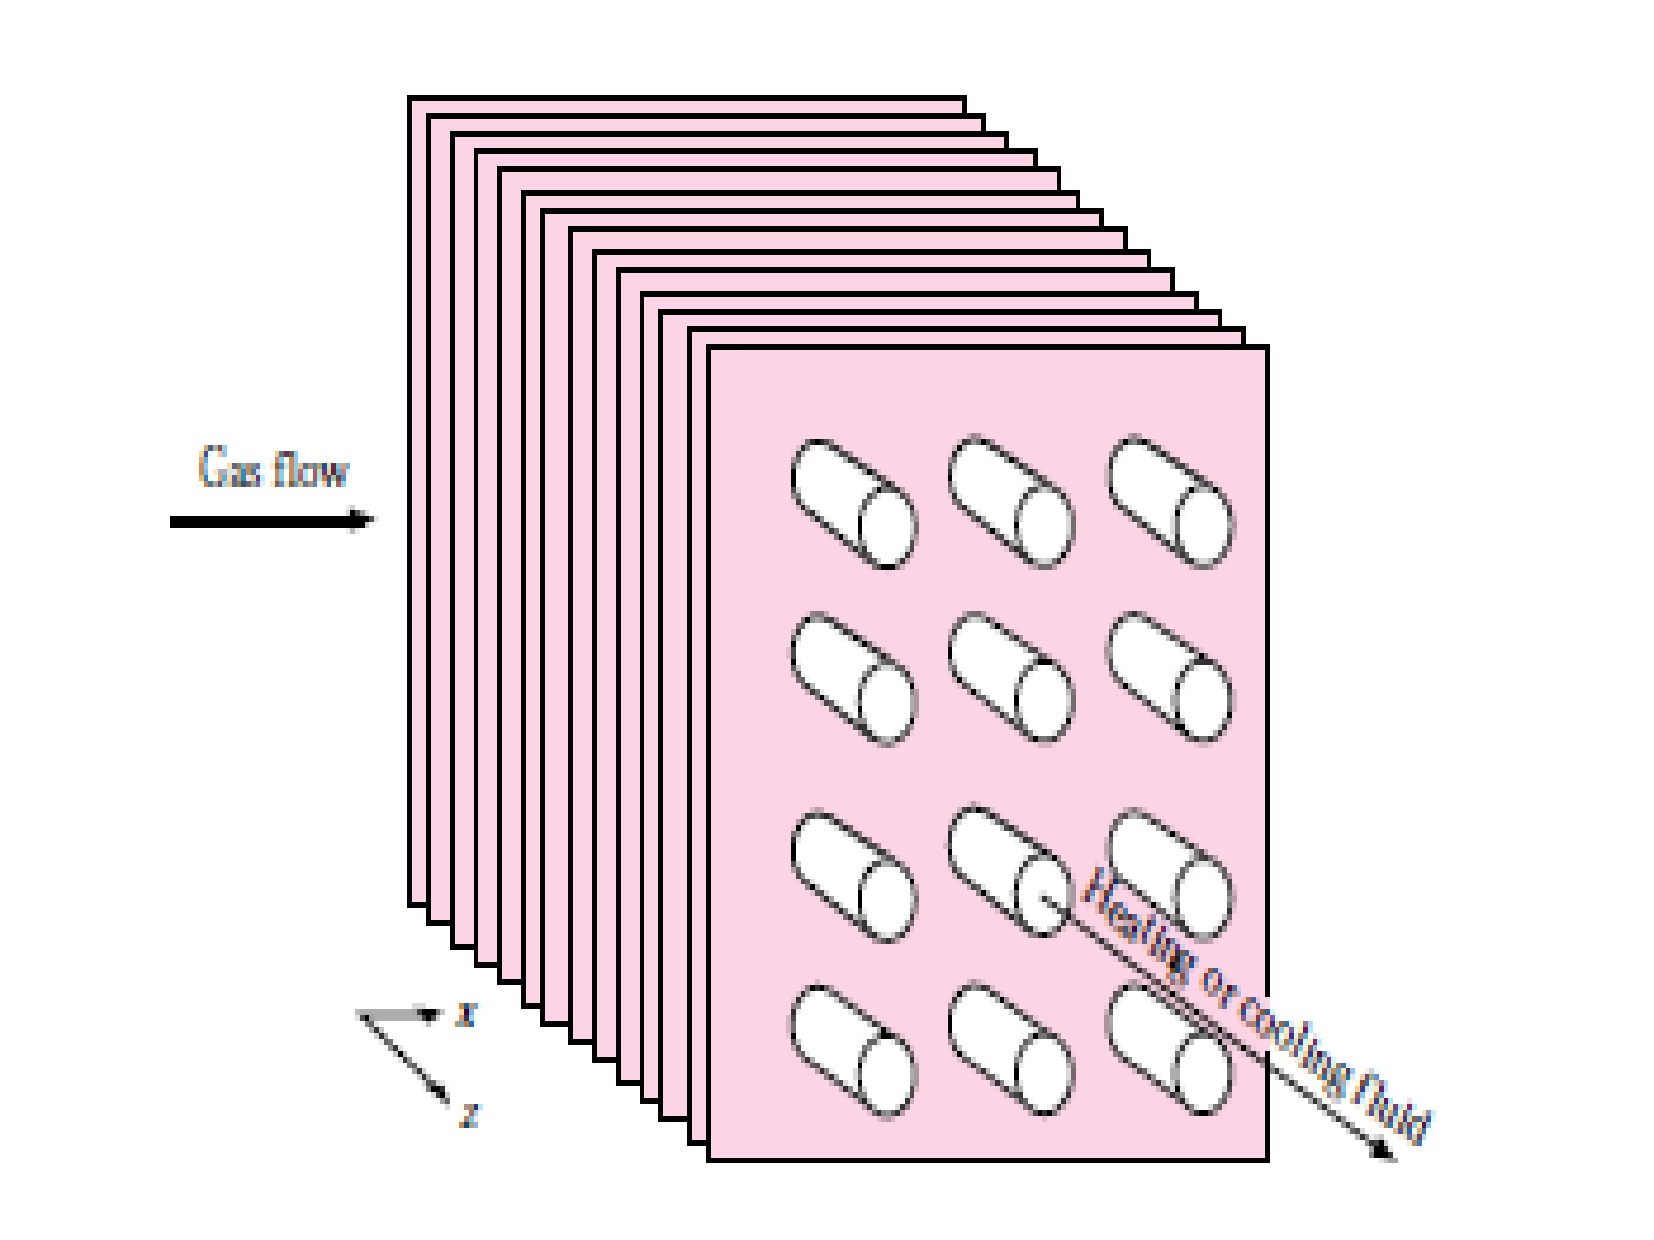
\includegraphics[width=1.1\columnwidth,clip]{./Pics/CrossFlowHE_UnmixedFluids_Example}
        \caption{Cross-flow HE with Unmixed fluids (~\ref{Problem:HE_Example5}).}\label{Fig:XFlow}
   \end{figure}
\end{center}



%%% (Cengel 13.18)
\item\label{Problem:HE_Cengel13_18} A double-pipe heat exchanger is constructed of a copper ($\kappa=$ 380 W/(m.$^{\circ}$C) inner tube of internal diameter $D_{i}=$ 1.2 cm and external diameter $D_{o}=$ 1.6 cm and an outer tube of diameter 3.0 cm. The convection heat transfer coefficient is $h_{i}=$ 700 W/(m$^{2}.^{\circ}$C) on the inner surface of the tube and $h_{o}=$ 1400 W/(m$^{2}.^{\circ}$C) on its outer surface. For a fouling factor $R_{f,i}=$ 0.0005 m$^{2}.^{\circ}$C/W on the tube side and $R_{f,o}=$ 0.0002 m$^{2}.^{\circ}$C/W on the shell side. Determine 
\begin{enumerate}
   \item the thermal resistance of the heat exchanger per unit length and,
   \item the overall heat transfer coefficients $U_{i}$ and $U_{o}$ based on the inner and outer surface areas of the tube, respectively.
\end{enumerate}


%%% Cengel 13.64
\item\label{Problem:HE_Cengel13_64} In a binary geothermal power plant, the working fluid isobutane is condensed by air in a condenser at 75$^{\circ}$C $\left(h_{\text{fg}}=\text{ 255.7 kJ/kg}\right)$ at a rate of 2.7 kg/s. Air enters the condenser at 21$^{\circ}$C and leaves at 28$^{\circ}$C. The heat transfer surface area based on the isobutane side is 24 m$^{2}$. Determine the mass flow rate of air and the overall heat transfer coefficient.



%%% Cengel 13.89
\item\label{Problem:HE_Cegel13_89} A cross-flow air-to-water heat exchanger with an effectiveness of 0.65 is used to heat water ($C_{p}=$ 4180 J/(kg.$^{\circ}$C) with hot air  ($C_{p}=$ 1010 J/(kg.$^{\circ}$C). Water enters the heat exchanger at 20$^{\circ}$C at a rate of 4 kg/s, while air enters at 100$^{\circ}$C at a rate of 9 kg/s. If the overall heat transfer coefficient based on the water side is 260 W/(m$^{2}.^{\circ}$C), determine the heat transfer surface area of the heat exchanger on the water side. Assume both fluids are unmixed.


%%% Cengel 13.107
\item\label{Problem:HE_Cegel13_107} A shell-and-tube process heater is to be selected to heat water ($C_{p}=$ 4180 J/(kg.$^{\circ}$C) from 20$^{\circ}$C to 90$^{\circ}$C by steam flowing on the shell side. The heat transfer load of the heater is 600 kW. If the inner diameter of the tubes is 1 cm and the velocity of water is not to exceed 3 m/s, determine how many tubes need to be used in the heat exchanger.


%%%%
\end{enumerate}



\clearpage

%{
%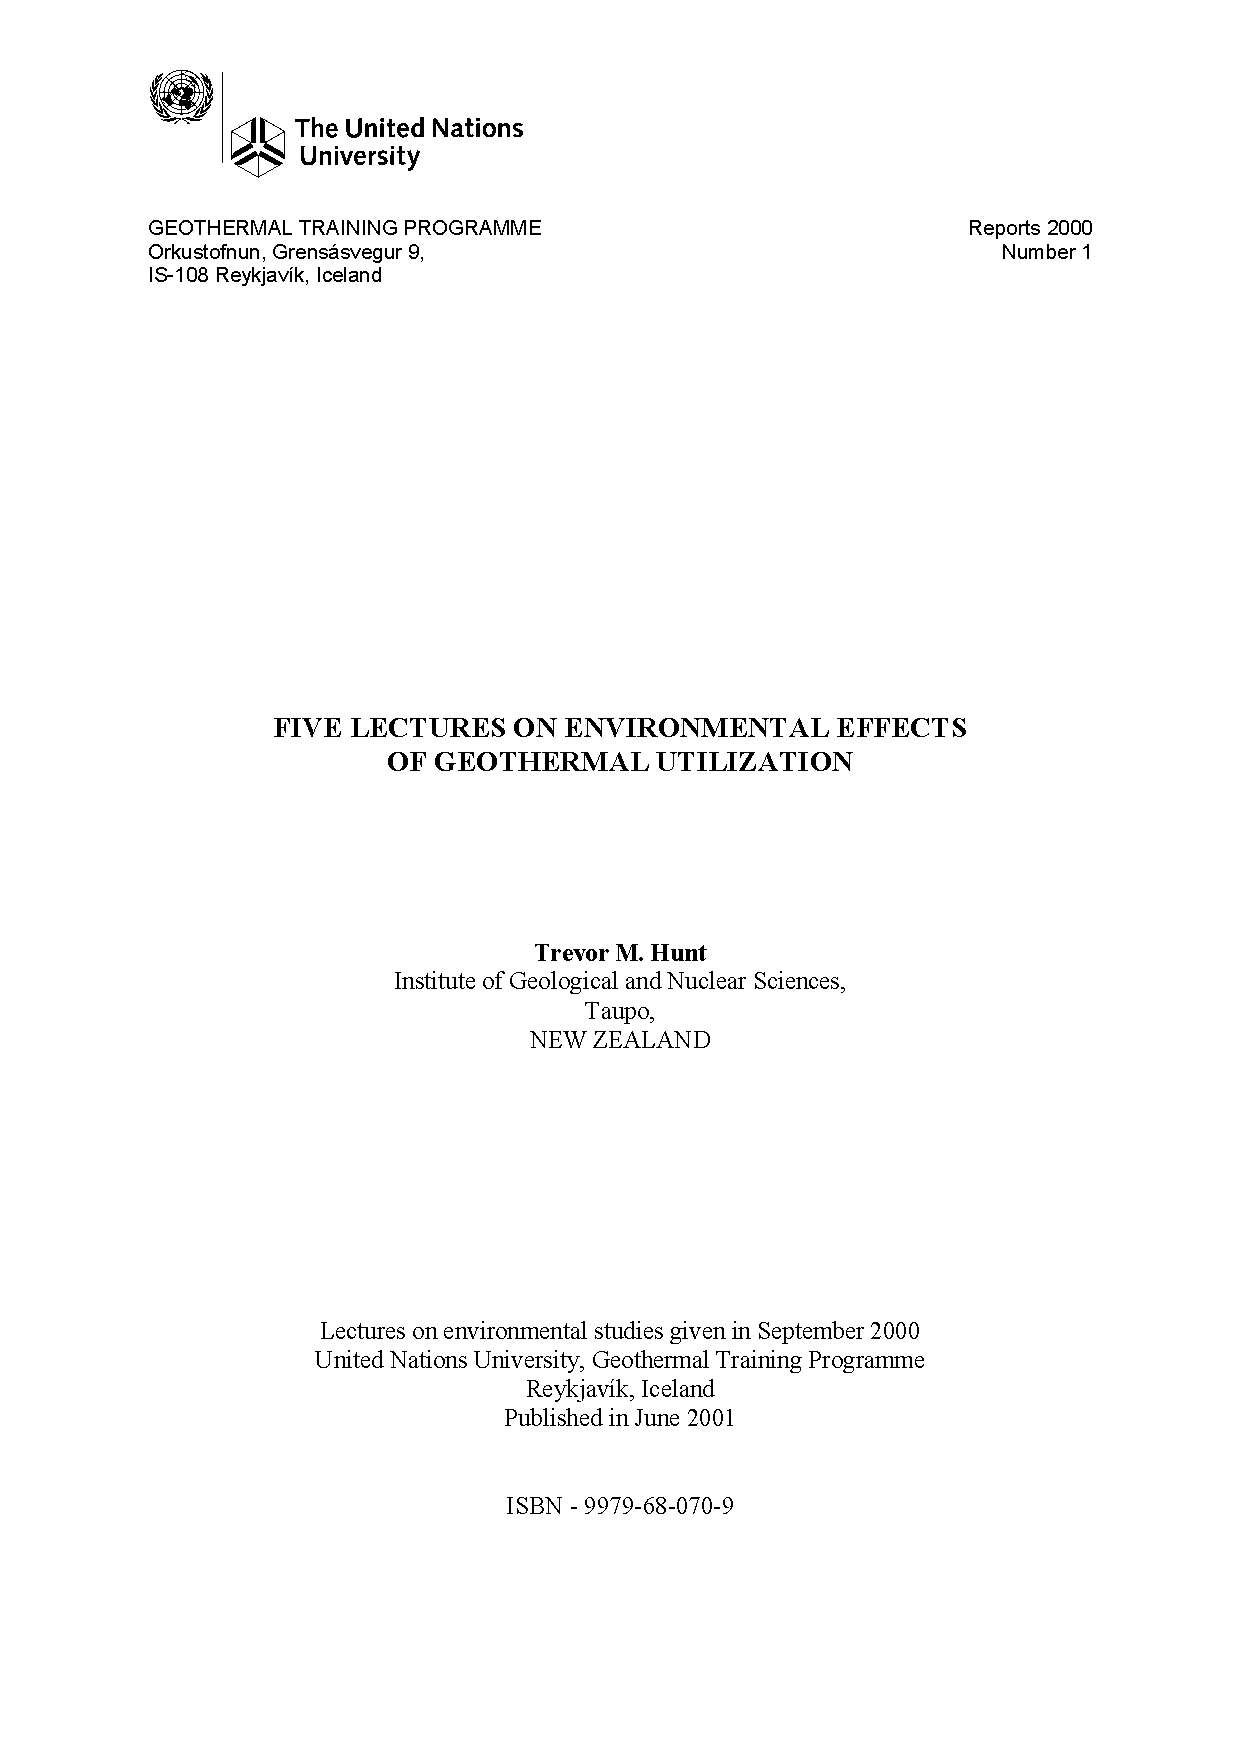
\includepdf[pages=-,fitpaper, angle=0]{./HuntSelect.pdf}
%}

\end{document}
